\documentclass{beamer}
\mode<presentation> 
\usetheme{Warsaw}
\useinnertheme{rectangles}
\useoutertheme{infolines}
% centaur logo color: 174,191,219
\usecolortheme[RGB={134,151,179}]{structure}
\definecolor{Highlight}{rgb}{0,0,1}
\newcommand{\Highlight}[1]{{\color{Highlight}#1}}
\logo{\includegraphics[scale=0.31]{logo}} 

\beamertemplatenavigationsymbolsempty


\usebeamerfont{title}
\usebeamerfont{author}
\usebeamerfont{institute}
\usebeamerfont{date}
\title{A Verilog Parser in ACL2}
\author[Page \thepage]{Jared Davis}
\institute{Centaur Technology}
\date{September 10, 2008}
\setlength{\parindent}{0pt}
\newcommand{\SmallSkip}{\vspace{0.5cm}\noindent}
\newcommand{\Skip}{\vspace{1cm}\noindent}
\newcommand{\MedSkip}{\vspace{1.5cm}\noindent}
\newcommand{\BigSkip}{\vspace{2cm}\noindent}
\begin{document}
\maketitle
\logo{}


\section[Introduction]{}
\begin{frame}
\frametitle{Introduction}
A preprocessor, lexer, and parser for Verilog 2005 (IEEE-1364)
\begin{itemize}
\item Basically complete for modules
\end{itemize}
\SmallSkip
Verilog is a pretty big language
\begin{itemize}
\item Long history, many-level modelling, simulation mixed in
\item Preprocessor, 125 keywords, 50 other token types, 20-page grammar
\end{itemize}
\SmallSkip
Primary concern: \Highlight{correct translation}
\begin{itemize}
\item Simplicity over performance
\item Elaborate well-formedness checks
\item Mostly in logic-mode with verified guards
\item Unit tests to promote semantic correctness
\end{itemize}
\end{frame}

\begin{frame}
\frametitle{High-level design}
\begin{center}
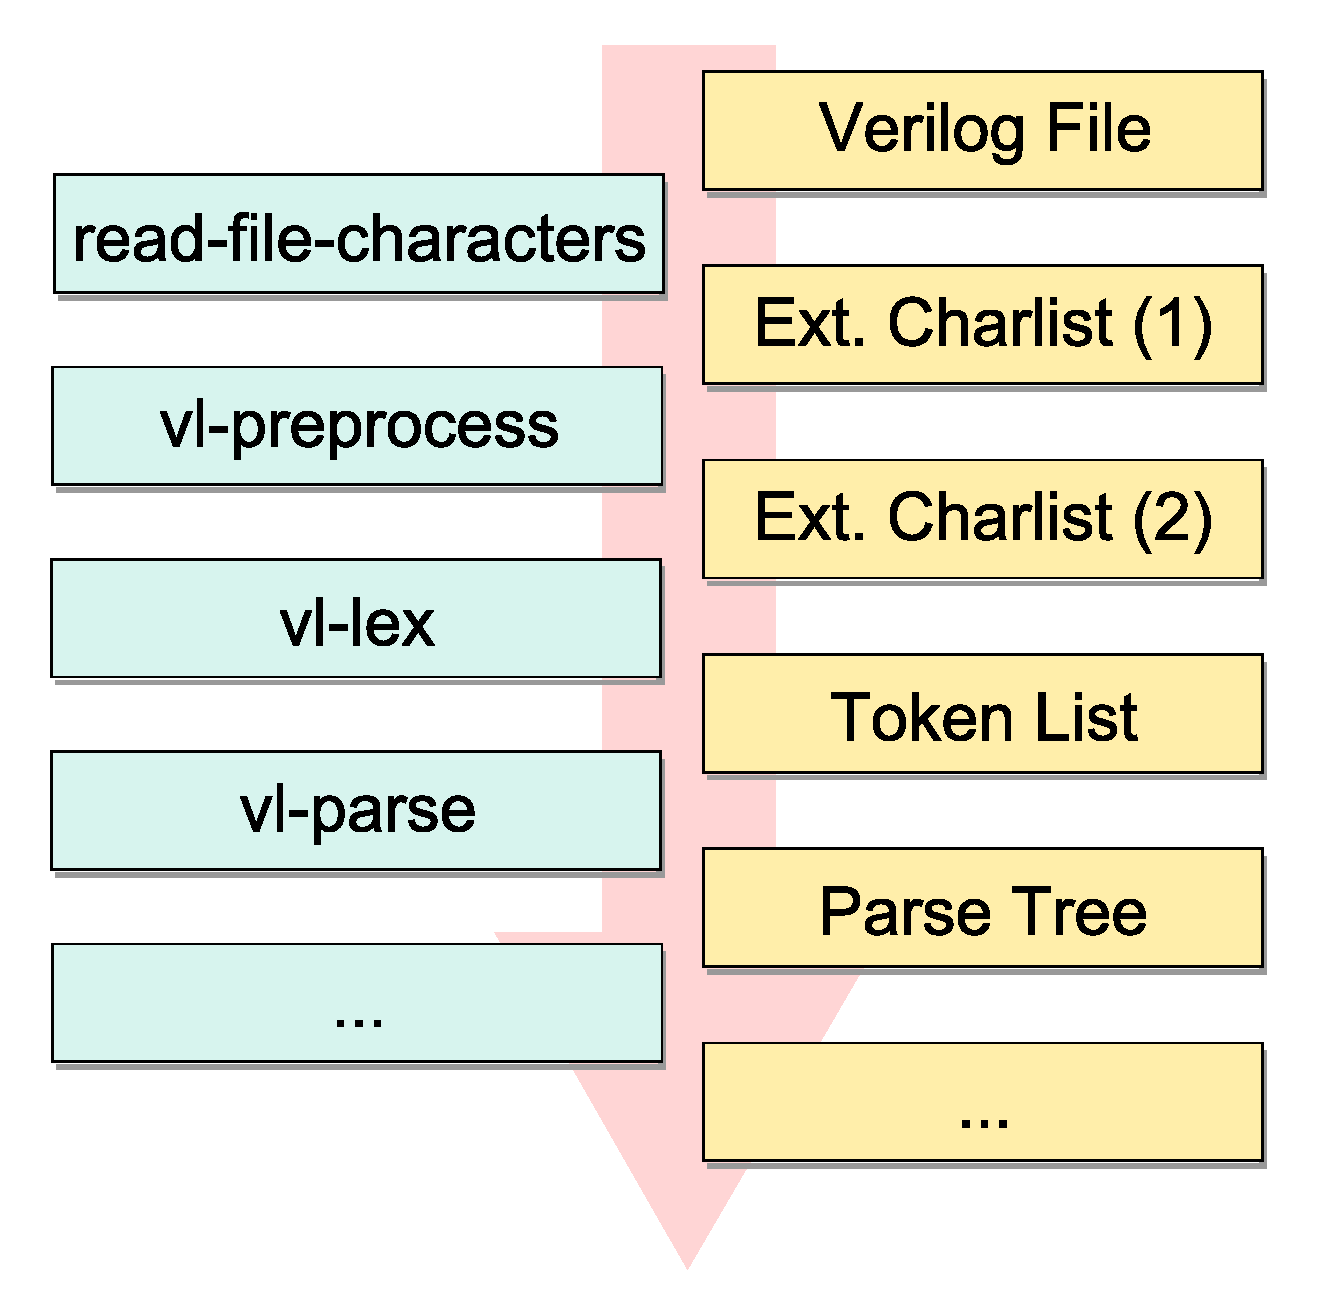
\includegraphics[scale=0.35]{vl-parser}
\end{center}
\end{frame}

\begin{frame}
\frametitle{Results}

Performance is quite acceptable (550K LOC)
\begin{center}
\begin{tabular}{lll}
Read top.v & 6s & 2.6 GB \\
Preprocess top.v & 4s & 1 GB \\
Lex top.v & 28s & 2.5 GB  \\
Parse top.v & 20s & 1.4 GB \\
Load libraries & 20s & 1.7 GB \\
\hline
Total & 78s & 9.3 GB
\end{tabular}
\end{center}

\SmallSkip
Working on making an ACL2 image with the chip pre-loaded

\end{frame}

\begin{frame}{Outline}
  \tableofcontents
\end{frame}


\section[Reading files]{Reading files}
\begin{frame}[fragile]
\frametitle{Reading files}

Verilog sources are just ASCII text files

\SmallSkip
We read in whole files as lists of \Highlight{extended characters}
\begin{itemize}
\item $\langle character, filename, line, column \rangle$
\end{itemize}

\SmallSkip
Inefficient, but has advantages:
\begin{itemize}
\item Minimizes use of state
\item Automatic position tracking
\item Easy to write tests for list-based tools
\end{itemize}

\end{frame}


\section[The preprocessor]{The preprocessor}
\begin{frame}[fragile]
\frametitle{The preprocessor}

Verilog has a C-style preprocessor
\begin{itemize}
\item define and undef for constants
\item nestable ifdef, ifndef, elsif, else
\item other stuff that we don't support (like include)
\end{itemize}

\SmallSkip
{\bf vl-preprocess} : echarlist $\rightarrow$ successp $\times$ echarlist
\begin{itemize}
\item Program mode
\item Reuses some lexer routines
\item 1,200 lines (about 45\% comments and whitespace)
\item Includes 250 lines of unit tests
\end{itemize}

\end{frame}

\begin{frame}[fragile]
\frametitle{Preprocessor implementation}

Woefully \Highlight{underspecified}, so we try to defensively mimic Cadence
\begin{verbatim}
`ifdef foo                        `define a 0
`define myendif `endif            `define b `a
`myendif                          `define a 1
                                  wire w = `b ;
\end{verbatim}

Not a blind textual substitution
\begin{verbatim}
  // comment about `ifdef 
  $display("The value of `a' is %d\n", a);
\end{verbatim}

\SmallSkip
No nice way to relate input and output

\end{frame}



\section[The lexer]{The lexer}
\begin{frame}
\frametitle{The lexer}

The lexer is quite basic.
\begin{itemize}
\item ``Optimized'' based on the first-remaining character
\item Verilog is pretty amenable to this
\end{itemize}

\SmallSkip

{\bf vl-lex} : echarlist $\rightarrow$ successp $\times$ tokenlist

\begin{itemize}
\item A mixture of program and logic mode
\item 1400 lines (about 40\% comments and whitespace)
\item Includes 400 lines of unit tests
\item About 40\% is related to numbers
\end{itemize}

\SmallSkip
Written with some ``theorems'' in mind:
\begin{itemize}
\item tokenlistp(output)
\item flatten(output) = input
\end{itemize}

\end{frame}



\begin{frame}
\frametitle{Token definition}

Our lexer produces a list of {\em tokens}.
\begin{itemize}
\item Plain tokens (ws, comments, operators, punctuation, keywords)
\item String, real, and integer literals
\item Identifiers and system identifiers
\end{itemize}

\SmallSkip
Each token has
\begin{itemize}
\item A symbolic type (which can be accessed quickly)
\item The echars the lexer created it from
\end{itemize}

\SmallSkip 

We have some basic well-formedness checks, e.g., an integer literal
should be in the specified range.

\end{frame}



\begin{frame}
\frametitle{Lexer utilities: literals}

Reasonably-efficient utilities for handling literals
\begin{itemize}
\item {\bf vl-matches-string-p} : string $\times$ echars $\rightarrow$ bool
\item {\bf vl-read-literal} : string $\times$ echars $\rightarrow$ prefix $\times$ remainder
\item {\bf vl-read-some-literal} : strings $\times$ echars $\rightarrow$ prefix $\times$ remainder
\item {\bf vl-read-until-literal} : string $\times$ echars $\rightarrow$ bool $\times$ prefix $\times$ remainder
\item {\bf vl-read-through-literal} : string $\times$ echars $\rightarrow$ bool $\times$ prefix $\times$ remainder
\end{itemize}

\SmallSkip
We also prove some basic theorems about these
\end{frame}



\begin{frame}[fragile]
\frametitle{Lexer utilities: defchar}

\SmallSkip
We also automate the introduction of character types.  For instance:
\begin{verbatim}
(defchar whitespace 
  (or (eql x #\Space)
      (eql x #\Tab)
      (eql x #\Newline)
      (eql x #\Page)))
\end{verbatim}

Introduces efficient functions (w/ theorems):
\begin{itemize}
\item {\bf vl-whitespace-p} : characterp $\rightarrow$ bool
\item {\bf vl-whitespace-echar-p} : echar $\rightarrow$ bool
\item {\bf vl-whitespace-list-p} : character-listp $\rightarrow$ bool
\item {\bf vl-read-while-whitespace} : echars $\rightarrow$ nil $\times$ prefix $\times$ remainder
\end{itemize}
\end{frame}






\section[Classic recursive-descent parsing]{Classic recursive-descent parsing}
\begin{frame}[fragile]
\frametitle{Classic recursive-descent parsing}

\[
\mathit{range} ::= \textbf{[} \; \mathit{expression} \; \textbf{:} \; \mathit{expression} \; \textbf{]}
\]
{\small
\begin{verbatim}
File in;

Token match_token(type) {
   Token t = lex();
   if (t.getType() == type) return t;
   throw new Exception("Expected " + type);
}

Range parse_range() {
   match_token(LBRACK);
   Expression e1 = parse_expression();
   match_token(COLON);
   Expression e2 = parse_expression();
   match_token(RBRACK);
   return new Range(e1, e2);
}
\end{verbatim}}
\end{frame}

\begin{frame}

\frametitle{Observations}

A reasonable way to write parsers
\begin{itemize}
\item follows the grammar rule quite closely
\item implicitly propagates errors upwards (nice)
\item implicitly advances through the file (nice)
\end{itemize}

\SmallSkip

Let me emphasize these last two points:
\begin{itemize}
\item parse\_range can fail (by propagating an exception)
\item parse\_range changes state (the file pointer)
\end{itemize}

\SmallSkip

\Highlight{Not straightforward} to do in ACL2.

\end{frame}


\begin{frame}[fragile]
\frametitle{Explicit state and exception handling = pain}

{\small
\begin{verbatim}
(defun parse-range (tokens)
  (mv-let (err val tokens) (match-token :LBRACK tokens)
   (if err
       (mv err val tokens)
     (mv-let (err e1 tokens) (parse-expression tokens)
      (if err
          (mv err e1 tokens)
        (mv-let (err val tokens) (match-token :COLON tokens)
         (if err
             (mv err val tokens)
           (mv-let (err e2 tokens) (parse-expression tokens)
            (if err
                (mv err e2 tokens)
              (mv-let (err val tokens) (match-token :RBRACK tokens)
               (if err
                   (mv err val tokens)
                 (mv nil (make-range e1 e2) tokens))))))))))))
\end{verbatim}
}

\end{frame}

\section[The SEQ language]{The SEQ language}
\begin{frame}[fragile]
\frametitle{The SEQ language}

SEQ is a macro-language for writing parsers
\begin{itemize}
\item Makes exception-propagation implicit
\item Makes advancing the token list implicit
\end{itemize}

\begin{verbatim}
(defun parse-range (tokens)
  (declare (xargs :guard (tokenlistp tokens)))
  (seq tokens
     (:= (match-token :LBRACK tokens))
     (e1 := (parse-expression tokens))
     (:= (match-token :COLON tokens))
     (e2 := (parse-expression tokens))
     (:= (match-token :RBRACK tokens))
     (return (make-range e1 e2))))
\end{verbatim}

\end{frame}


\begin{frame}[fragile]
\frametitle{Actions and streams}
SEQ is a language for applying {\em actions} to a {\em stream}.

\SmallSkip
Actions are ACL2 expressions which return
\[
\texttt{(mv} \; \mathit{error} \; \mathit{val} \; \mathit{stream}' \texttt{)}
\]
Where
\begin{itemize}
\item $\mathit{error}$ is non-nil if an error has occurred,
\item $\mathit{val}$ is the return value of this action
\item $\mathit{stream'}$ is the updated stream
\end{itemize}

\SmallSkip
Streams are basically any ACL2 object you wish to sequentially update
\end{frame}




\begin{frame}[fragile]
\frametitle{SEQ language: returns}

Every seq program must end with a return statement.

\SmallSkip

{\bf Successful returns}

\begin{verbatim}
(return (foo ...))
  --->
(mv nil (foo ...) streamname)
\end{verbatim}

{\bf Raw returns}

\begin{verbatim}
(return-raw (mv "Bad!" nil streamname))
  --->
(mv "Bad!" nil streamname)
\end{verbatim}
\end{frame}


\begin{frame}[fragile]
\frametitle{SEQ language: voids}
{\bf Void Statements} can update the stream and cause errors

\SmallSkip
\begin{verbatim}
(:= (action ... args ...))
... more statements ...
 --->
(mv-let ([err] [val] streamname)
        (action ... args ...)
        (if [err]
            (mv [err] [val] streamname)
          (check-not-free ([err] [val])
             ... more statements ...)))
\end{verbatim}
\end{frame}


\begin{frame}[fragile]
\frametitle{SEQ language: simple binds}
{\bf Simple Binds} can update the stream, cause errors, and bind a name

\SmallSkip
\begin{verbatim}
(foo := (action ... args ...))
... more statements ...
 --->
(mv-let ([err] foo streamname)
        (action ... args ...)
        (if [err]
            (mv [err] foo streamname)
          (check-not-free ([err])
             ... more statements ...)))
\end{verbatim}
\end{frame}



\begin{frame}[fragile]
\frametitle{SEQ language: destructuring binds}
{\bf Destructuring Binds} can update the stream, cause errors, and bind many names

\SmallSkip
\begin{verbatim}
((foo . bar) := (action ... args ...))
... more statements ...
 --->
(mv-let ([err] [val] streamname)
        (action ... args ...)
        (if [err]
            (mv [err] [val] streamname)
          (let ((foo (car [val]))
                (bar (cdr [val])))
             (check-not-free ([err] [val])
                ... more statements ...))))
\end{verbatim}
\end{frame}


\begin{frame}[fragile]
\frametitle{SEQ language: when and unless}
{\bf When/Unless Blocks} are useful for matching optional stuff
\[
\mathit{inoutdecl} ::= {\bf inout} \; \mathit{nettype} \; [{\bf signed}] \; [\mathit{range}] \; \mathit{list\_of\_port\_identifiers}
\]

\begin{verbatim}
(seq tokens
     (:= (match-token :kwd-inout tokens))
     (type := (parse-net-type tokens))
     (when (is-token :kwd-signed tokens)
       (signed := (match-token :kwd-signed tokens)))
     (when (is-token :lbrack tokens)
       (range := (parse-range tokens)))
     (ids := (parse-list-of-port-ids tokens))
     (return (make-inoutdecl type signed range ids)))
\end{verbatim}

\end{frame}

\begin{frame}[fragile]
\frametitle{SEQ language: early returns}
{\bf Early Returns} are useful for choosing between alternative productions.
\[
\mathit{nonempty\_list\_of\_ids} ::= \mathit{identifier} \; \{ \; {\bf ,} \; \mathit{identifier} \; \} 
\]
\begin{verbatim}
(defun parse-nonempty-list-of-ids (tokens)
  (seq tokens
       (first := (match-token :identifier tokens))
       (unless (is-token :comma tokens)
         (return (list first)))
       (:= (match-token :comma tokens))
       (rest := (parse-nonempty-list-of-ids tokens))
       (return (cons first rest))))
\end{verbatim}
\end{frame}

\begin{frame}[fragile]
\frametitle{SEQ language: looking ahead}

{\bf Arbitrary lookahead} is trivial when you are traversing a list.  For
stobjs, you would need some kind of unget operation.

{\small
\begin{verbatim}
(defun parse-nonempty-list-of-ids (tokens)
  (seq tokens 
       (first := (match-token :identifier tokens))
       (when (and (is-token :comma tokens)
                  (is-token :identifier (cdr tokens)))
         (:= (match-token :comma tokens))
         (rest := (parse-nonempty-list-of-ids tokens)))
       (return (cons first rest))))
\end{verbatim}}
\end{frame}


\begin{frame}[fragile]
\frametitle{SEQ language: backtracking}

{\bf Backtracking} is also relatively straightforward by "trapping" errors.

{\small 
\begin{verbatim}          
(defun parse-foo-or-bar (tokens)
  (mv-let (erp foo updated-tokens)
          (parse-foo tokens)
          (if (not erp)
              (mv nil foo updated-tokens)
            (parse-bar tokens))))

(defun parse-foo-or-bar (tokens)
  (seq-backtrack tokens
                 (parse-foo tokens)
                 (parse-bar tokens)))
\end{verbatim}}
\end{frame}


\section{Final touches}
\begin{frame}[fragile]
\frametitle{Sensible error reporting for primitives}

My {\bf match-token} and {\bf is-token} are macros instead of functions.

\SmallSkip
For error reporting, we can introduce our parsing functions with {\bf defparser} 
instead of defun.

\begin{verbatim}
(defparser foo (... tokens) 
  body)
 --->
(defun foo (... tokens)
  (let ((__function__ 'foo))
    (declare (ignorable __function__))
    body))
\end{verbatim}

\end{frame}

\begin{frame}[fragile]
\begin{verbatim}
(defmacro is-token (type &optional (tokens 'tokens))
  (declare (xargs :guard (tokentypep type)))
  `(and (consp ,tokens)
        (eq (token-type (car ,tokens)) ,type)))

(defmacro match-token (type &optional (tokens 'tokens))
  (declare (xargs :guard (tokentypep type)))
  (let ((tokens ,tokens))
       (if (not (consp tokens))
           (mv [[error in __function__, unexpected eof ]] 
               nil tokens)
         (let ((token1 (car tokens)))
           (if (not (eq ,type (token-type token1)))
               (mv [[error in __function__ at [place] ...]]
                   nil tokens)
           (mv nil token1 (cdr tokens)))))))
\end{verbatim}
\end{frame}



\begin{frame}[fragile]
\frametitle{Efficiency note}
Creating error strings was really slow.

\SmallSkip 
Consing together error structures instead reduced parser time by
80\% even though there isn't that much backtracking.

{\small
\begin{verbatim}
(list "foo is ~x0 and bar is ~x1.~%" foo bar)
  vs.
(concatenate 'string "foo is " 
             (coerce (explode-atom foo 10) 'string)
             "and bar is "
             (symbol-name bar)
             ".~%")
\end{verbatim}}
\end{frame}


\begin{frame}[fragile]
\frametitle{More syntactic sugar}

{\tt Defparser} generates a macro alias with implicit tokens

And automates the {\tt tokenlistp} guard

\begin{verbatim}
(defparser parse-range (tokens)
  (seq tokens
       (:= (match-token :LBRACK))
       (e1 := (parse-expression))
       (:= (match-token :COLON))
       (e2 := (parse-expression))
       (:= (match-token :RBRACK))
       (return (make-range e1 e2))))

(defparser parse-foo (tokens)
  (seq tokens
       (range := (parse-range))
       ...))
\end{verbatim}

\end{frame}




\section{Logic-mode parsing}
\begin{frame}[fragile]
\frametitle{Logic-mode parsing}

With 170 defparser functions, we need to automate theorem creation.

\SmallSkip
We classify our parsers as having various properties, and use these
properties to decide what theorems to prove about them.

\SmallSkip
Sometimes, combinations of properties can lead to better theorems.

\SmallSkip
Net effect: logic mode and guard verification are fairly easy.
\end{frame}


\begin{frame}[fragile]
\frametitle{Termination behavior}

Every defparser we've written is at least {\bf weakly decreasing}:
\begin{itemize}
\item {\small\begin{verbatim}
(<= (acl2-count (third (parse-foo)))
    (acl2-count tokens))
\end{verbatim}}
\end{itemize}

\SmallSkip
Most are also {\bf strongly decreasing}:
\begin{itemize}
\item {\small\begin{verbatim}
(implies (not (first (parse-foo)))
         (< (acl2-count (third (parse-foo)))
            (acl2-count tokens)))
\end{verbatim}}
\end{itemize}

\SmallSkip
While some others are only {\bf strong on value}:
\begin{itemize}
\item {\small\begin{verbatim}
(implies (second (parse-foo))
         (< (acl2-count (third (parse-foo)))
            (acl2-count tokens)))
\end{verbatim}}
\end{itemize}

\end{frame}


\begin{frame}[fragile]
\frametitle{Failure behavior}

Most (all?) of our parsers fail {\bf gracefully}:
\begin{itemize}
\item {\small\begin{verbatim}
(implies (first (parse-foo))
         (not (second (parse-foo))))
\end{verbatim}}
\end{itemize}

\SmallSkip
But some {\bf never} fail: (e.g., optional or zero+ productions)
\begin{itemize}
\item {\small\begin{verbatim}
(not (first (parse-foo)))
\end{verbatim}}
\end{itemize}

\end{frame}




\begin{frame}[fragile]
\frametitle{Result characterization}

On success, we usually have some idea what the {\bf result} ought to be:
\begin{itemize}
\item {\small\begin{verbatim}
(implies (and (not (first (parse-foo)))
              ...guards...)
         (foop (second (parse-foo))))
\end{verbatim}}
\end{itemize}

\SmallSkip
We've also found it useful to know if the result is a {\bf true-listp}.
\begin{itemize}
\item {\small\begin{verbatim}
(true-listp (second (parse-foo)))
\end{verbatim}}
\end{itemize}

\SmallSkip It's also useful to know if {\bf resultp-of-nil} is true.
\begin{itemize}
\item If {\tt (foop nil)} and fails gracefully, omit first hyp.
\item If never fails, omit first hyp.
\end{itemize}

\end{frame}



\begin{frame}[fragile]
\frametitle{Actual examples (verbatim)}

{\small
\begin{verbatim}
(defparser vl-parse-range (tokens)
  :result (vl-range-p val)
  :resultp-of-nil nil
  :fails gracefully
  :count strong
  (seq tokens
       (:= (vl-match-token :vl-lbrack))
       (left := (vl-parse-expression))
       (:= (vl-match-token :vl-colon))
       (right := (vl-parse-expression))
       (:= (vl-match-token :vl-rbrack))
       (return (vl-range left right))))
\end{verbatim}}
\end{frame}

\begin{frame}[fragile]
\frametitle{Actual examples (verbatim)}

{\small
\begin{verbatim}
(defparser vl-parse-optional-drive-strength (tokens)
  :result (vl-maybe-gatestrength-p val)
  :resultp-of-nil t
  :fails never
  :count strong-on-value
  (mv-let (erp val explore)
          (vl-parse-drive-strength)
          (if erp
              (mv nil nil tokens)
            (mv nil val explore))))
\end{verbatim}}

\end{frame}


\begin{frame}[fragile]
\frametitle{Actual examples (verbatim)}

{\small
\begin{verbatim}
(defparser vl-parse-list-of-param-assignments (tokens)
  :result (vl-param-assignment-tuple-list-p val)
  :resultp-of-nil t
  :true-listp t
  :fails gracefully
  :count strong
  (seq tokens
       (first := (vl-parse-param-assignment))
       (when (vl-is-token? :vl-comma)
         (:= (vl-match-token :vl-comma))
         (rest := (vl-parse-list-of-param-assignments)))
       (return (cons first rest))))
\end{verbatim}}
\end{frame}


\begin{frame}[fragile]
\frametitle{Mutual recursion termination problems}

We can't expand definitions of mutually-recursive functions until they've
been admitted, so this doesn't work:

{\small
\begin{verbatim}
(vl-mutual-recursion 
 (defparser vl-parse-lvalue (tokens) 
   ...)

 (defparser vl-parse-list-of-lvalues (tokens)
   (declare ...)
   (seq tokens
        (first := (vl-parse-lvalue))
        ...
        (rest := (vl-parse-list-of-lvalues tokens))
        ...))
\end{verbatim}}

We hackishly extend SEQ with \Highlight{:s=} and \Highlight{:w=} to address this.

\end{frame}



\section{The parser}

\begin{frame}[fragile]
\frametitle{The parser}

{\bf vl-parse} : tokenlist $\rightarrow$ successp $\times$ modulelist
\begin{itemize}
\item Entirely logic mode, guards verified
\item 7,800 lines (more than half comments/whitespace)
\item 1,400 lines of unit tests (want more)
\item Almost $\frac{1}{3}$ deals with expressions and statements (mutual recursion)
\end{itemize}

\SmallSkip
Similar to Terry's original parser (Common Lisp)
\begin{itemize}
\item Loop is about the only thing seq doesn't handle well
\item Backtracking is quite nice
\end{itemize}

% 7800 total 1270 comments, 3511 ws
% blockitems:  1044 - 454 = 590
% delays: 210 - 138 = 72 
% expr : 1740 - 1459 = 281
% nets : 707 - 399 = 308
% ports: 413 - 352 = 61
% ranges: 128 - 92 = 36
% strengths: 207 - 153 = 54
% 1402 lines


\end{frame}


\begin{frame}[fragile]
\frametitle{Parse trees}

We introduce parse trees in a separate file (parsetree.lisp) which has few
dependencies.

\SmallSkip
Mostly we just introducing various aggregates, for instance:

{\small
\begin{verbatim}
(defaggregate regdecl
 (name signedp range arrdims initval atts)
 :tag :regdecl
 :require
 ((stringp-of-regdecl->name         (stringp name))
  (booleanp-of-regdecl->signedp     (booleanp signedp))
  (maybe-range-p-of-regdecl->range  (maybe-range-p range))
  (rangelist-p-of-regdecl->arrdims  (rangelist-p arrdims))
  (maybe-expr-p-of-regdecl->initval (maybe-expr-p initval))
  (atts-p-of-regdecl->atts          (atts-p atts))))
\end{verbatim}}
\end{frame}

\begin{frame}[fragile]
\frametitle{Parse tree implementation}

Defaggregate and deflist get me pretty far, but they don't do everything.
\begin{itemize}
\item Not useful in mutually-recursive cases
\item I need to write a good sum-of-products macro
\end{itemize}

\SmallSkip 
For now, some custom-written recognizers, constructors, and accessors to
handle these cases --- ugh!

\SmallSkip 2,100 lines (35\% ws/comments), all logic-mode, guards-verified, lots
of basic theorems (mostly automatic)

\SmallSkip Used by our translation process
\begin{itemize}
\item Completeness, non-conflicting names, reasonable constructs
\item Unparameterization, expression simplification, e-ification
\end{itemize}
\end{frame}



\section{Demo}

\begin{frame}[fragile]
\frametitle{Demo}

\end{frame}



\end{document}
